\documentclass{article}
\usepackage{graphicx}
\usepackage{amsthm}
\usepackage{amsmath}
\usepackage{amssymb}
\usepackage{tikz-cd}
\usepackage{etoolbox}

\usepackage{geometry}
 \geometry{
 a4paper,
 total={170mm,257mm},
 left=20mm,
 top=20mm,
 }

\let\oldproofname=\proofname
\renewcommand\proofname{\bf{\oldproofname}}
\renewcommand\qedsymbol{$\blacksquare$}

\theoremstyle{definition}
\newtheorem{thm}{Theorem}
\newtheorem{lemma}{Lemma}
\newtheorem{defn}{Definition}[section]

\newcommand{\notimplies}{%
  \mathrel{{\ooalign{\hidewidth$\not\phantom{=}$\hidewidth\cr$\implies$}}}}

\newcommand{\cat}{
	\mathbf
}
\newcommand{\domain}[1]{
	\mathrm{dom}(#1)
}
\newcommand{\codomain}[1]{
	\mathrm{cod}(#1)
}
\newcommand{\idarrow}[1][]{
	\mathrm{1}_{#1}
}

\AtBeginEnvironment{quote}{\singlespacing\small}

\setlength{\parskip}{1em}
\setlength{\parindent}{2em}

\graphicspath{{figures/}}


\begin{document}

\title{Casper research: \\ A Template for Correct-by-Construction Consensus Protocols \\ Featuring:\\ A specification of Casper the Friendly GHOST}
\maketitle

\begin{abstract}
We detail a process for generating correct-by-construction consensus protocols while providing language and ideas for reasoning about consensus protocols. Then we share the specifications of and experimental observations from two consensus protocols that are derived according to this method---one replicating a single bit, and another replicating a blockchain (i.e. Casper the Friendly GHOST).
\end{abstract}


\section{Part 0: Introduction}

Consensus protocols are used by nodes in distributed systems to decide on the same values, or on the same list of inputs to a replicated state machine (with irrevocable finality). There are, roughly speaking, two classes of consensus protocols known today. One we refer to as ``traditional consensus''. This class has its ``genetic roots'' in Paxos and multi-Paxos[CITE], and in the ``traditional'' consensus protocol research from the 80s and 90s[CITE]. The other we refer to as ``blockchain consensus''. These are protocols that have their roots in the Bitcoin blockchain and Satoshi Nakamoto's whitepaper[CITE]. We now discuss the differences between these classes of protocols, before giving an overview of the correct-by-construction process.

\subsection{Comparing Traditional Consensus to Blockchain Consensus}

Traditional consensus protocols (such as multi-Paxos and pbft) are notoriously difficult to understand[CITE (http://paxos.systems/)]. Blockchain consensus protocols, on the other hand, are much more accessible. This difference comes at least in part from the relative simplicity of Bitcoin's specification[CITE].

Traditional consensus protocols have (possibly ``hard-coded'') consensus on the set of nodes that can influence the execution of the protocol. In contrast, blockchain consensus protocols generally do not have consensus on the set of nodes that form consensus\footnote{Although Bitcoin and related protocols do not have consensus on a set of influencer nodes, they do not let anyone freely influence the execution of the protocol due to the computational difficulty of producing a valid block.}.

Checking message validity is a core component in blockchain consensus protocols, but this concept rarely makes an appearance in traditional consensus protocols.

In the context of state machine replication, traditional protocols decide in sequence on one ``block'' of state transitions/transactions to add to the shared operation log at a time.  To decide on a block, each node requires $\mathcal{O}(N)$ messages, where $N$ is the number of consensus-forming nodes.

Blockchain consensus protocols like Bitcoin do not finalize/decide on one block one at a time. In fact, the Bitcoin blockchain in particular does not make ``finalized decisions'' at all; blocks are ``orphaned'' if/when they are not in the highest total difficulty chain. However, if the miners are able to mine on the same blockchain, then the blocks that get deep enough into the blockchain won't be reverted (``orphaned''). Thus, block-depth serves as a proxy for finalization. In blockchain consensus protocols, each node only requires approximately one message, $\mathcal{O}(1)$, for every block(!).

Traditional consensus protocol research has focussed on producing protocols which are asynchronously safe (i.e.\ blocks won't be reverted due to arbitrary timing of future events) and live in asynchrony (or partial synchrony) (i.e.\ nodes eventually decide on new blocks). On the other hand, blockchain consensus protocols like the Bitcoin blockchain are safe and live (for unknown block-depth or ``confirmation count'') in a partially synchronous network.

Traditional Byzantine fault tolerant consensus protocols have precisely stated Byzantine fault tolerance numbers (often $n = 3f + 1$)[CITE]. On the other hand, it is less clear exactly how many faults (measured as a proportion of hashrate) blockchain consensus protocols can tolerate[CITE].

\subsection{Overview of the correct-by-construction process}

We now give a process for generating consensus protocols with consensus safety (in some conditions). The ``correct-by-construction'' process has two parts: 1) specifying data types and definitions that the protocol must satisfy to benefit from the implied results/theorems, and 2) ``filling in the blanks''---defining implementations of data structures that satisfy the types/definitions required by the proof. The more abstractly part (1) is specified, the more protocols there exist that satisfy the proof, but the more blanks there are to fill in part (2).

We first present the most abstract version of the core result that we rely on, using the most abstract definition of consensus protocols for which the theorem holds that we could come up with. Then we ``fill in the blanks'' by making assumptions about the objects involved in our initial definiton, thereby refining the abstract definition of consensus protocol, making it more concrete.

Through this process we introduce:

\begin{itemize}
\item the non-triviality property of consensus protocols 
\item a fixed known set of $n$ consensus-forming nodes (with protocol states which are themselves optionally $n$-tuples of protocol states)
\item asynchronous fault tolerance for a given number of Byzantine faults (if it's less than the total number of nodes)
%\item safety oracles for protocols where nodes have ``weights" and only their ``latest observed state'' determines how they effect protocol execution
\end{itemize}

At every step the original proof is still satisfied, while we have more information about the consensus protocols which can be generated to satisfy the growing definition given in this process. Once these proofs are in place, generating consensus protocols that satisfy them is relatively easy. Additionally, the proofs themselves happen to be quite elementary.

Following the description of the correct-by-construction process, specifications and experimental observations of a couple of protocols that were generated by this process are given. The second of these protocols, ``Casper the Friendly GHOST'' is a blockchain consensus protocol that can achieve asynchronous Byzantine fault tolerant consensus safety on each block with the network overhead of the Bitcoin blockchain---$\mathcal{O}(1)$ messages/block/node.

\section{Part 1: Abstract Consensus Safety Proof}

We now give an abstract consensus safety proof as the foundation of the correct-by-construction process. We provide the safety theorem in the most generic terms possible, so that we can generate as wide of an array of protocols as possible. We therefore say nothing in the consensus safety proof about the possible values of the consensus, $\cat{C}$.

We instead use propositions from some logic about values of the consensus, $\mathcal{L}_\cat{C}$. The propositions are either ``True'' or ``False'' of/for every possible value of the consensus. The logic has negation and boolean operators/transformations.

We have a notion of ``protocol states'' and ``protocol executions'', which is implemented by a category $\cat{\Sigma}$. Finally, the consensus protocol requires a map $\mathcal{E}$ called the ``estimator'' which maps protocol states to propositions in the logic about values of the consensus. These propositions, called ``estimates'', are understood to be ``guesses'' about the value of the consensus.

We use the ``looseness'' of the estimator to capture the ``forking'' behaviour of a blockchain consensus protocol, where, for example, a block could be reverted. Note, decisions can always be implemented by this map (it's possible for $\mathcal{E}$ to be ``monotonic''), but decisions cannot implement forking/non-monotonic estimators (because the set of decisions is monotonic by definition, but forking is not).

Therefore, in order to capture both potentially-forking estimates and certainly-final decisions we only consider protocols with estimators and ask whether/when \emph{hypothetical} decisions on estimates are consensus safe. I.e.,

\begin{quote}
``\emph{if} a node \emph{were} to make a decision on estimate $p$ at protocol state $\sigma$, then that node would have consensus safety with any other node \emph{hypothetically} making a decision on estimate $q$ at state $\sigma'$ (under some conditions)''
\end{quote}

or in the context of Bitcoin,

\begin{quote}
``\emph{if} my Bitcoin client were to decide on the block 7 confirmations deep, it would have consensus safety with your client, \emph{if} our clients used similar criteria to make decisions (with very high probability in a synchronous network with less than some amount of Byzantine hashrate).''
\end{quote}

So we define the ``estimate safety consensus protocol'' to be a tuple $(\cat{C}, \mathcal{L}_\cat{C}, \cat{\Sigma}, \mathcal{E})$. We first define these components using only the minimum constraints needed to present the safety proof with a reasonable degree of rigor. In this and the subsequent section, we then continue to refine[CITE $wikipedia.org/wiki/Refinement_(computing)$] the protocol definition, until anything satisfying it can plausibly be said to be a Byzantine fault tolerant, asynchronously safe consensus protocol. Finally, the example consensus protocols given in Part 3 are constructed to satisfy the definitions and, therefore, inherit the safety proof.

Now we present the components of the definition of ``estimate safety consensus protocols'', then we state and prove the consensus safety theorem, and then we refine the definition until anything satisfying the definition is reasonably a consensus protocol.

\vspace{5mm}

\begin{defn}[Estimate Safety Consensus Protocols: Part 1 of ?]

\begin{description}An \emph{estimate safety consensus protocol} consists of a tuple $(\cat{C}, \mathcal{L}_\cat{C}, \cat{\Sigma}, \mathcal{E})$, containing:

\begin{align*}
\cat{C}, & &&\text{the set of possible values of the consensus}\\
\mathcal{L}_\cat{C}, & &&\text{a logic with propositions, $props(\mathcal{L}_\cat{C})$, that are satisfied (or not) by the elements of $\cat{C}$}\\
\cat{\Sigma}, & &&\text{the category of protocol executions, with objects $ob(\cat{\Sigma})$ called ``protocol states''}\\
\mathcal{E} : ob(\cat{\Sigma}) \to props(\mathcal{L}_\cat{C}), & &&\text{a function called the ``estimator''}
\end{align*}

For now, we say nothing about the set of possible values of the consensus, $\cat{C}$.

The logic $\mathcal{L}_\cat{C}$, however, must have:

%Consider being more formal in the definition, and add
%\begin{align*}
%    &\sigma \to \sigma' &&\text{(introducing assumption)}   &&\text{(1)}\\ 
   

\begin{itemize}
\item a set of propositions, $props(\mathcal{L}_\cat{C})$, which somehow implement maps $p:\cat{C} \to \{True, False\}$, mapping all possible consensus values to ``True'' or ``False''
\item a negation operator $\neg: props(\mathcal{L}_\cat{C}) \to props(\mathcal{L}_\cat{C})$, such that for every $c \in \cat{C}$, $p(c)$ xor $\neg{p}(c)$
\item normally defined boolean algebra operators ``and" $\land$, ``or" $\lor$, and ``implies" $\Rightarrow$
\end{itemize}

Using the $\land$ operator, any number of propositions $p_1$, $p_2$, $p_3$\ldots, $p_n$ can be ``compressed'' into a single proposition $p_1 \land p_2 \land p_3\ldots \land p_n$ which is true if and only if each of the propositions is true.

The category of protocol states $\cat{\Sigma}$ is a category. No additional information about $\cat{\Sigma}$ is required for Step 1, but we define some properties and notation that are subsequently relevant:

\begin{itemize}
\item $ob(\cat{\Sigma})$, a set of objects called ``protocol states'': $\sigma_1$, $\sigma_2$, $\sigma_3$,\ldots
\item $mo(\cat{\Sigma})$, a set of morphisms called ``protocol executions'': $\tau_1$, $\tau_2$, $\tau_3$,\ldots
\item each execution maps a protocol state to a protocol state $\tau:ob(\cat{\Sigma}) \to ob(\cat{\Sigma})$
\item if a morphism $\tau$ maps object $\sigma_1$ to object $\sigma_2$, we write $\sigma_1 \xrightarrow[]{\tau} \sigma_2$
\item if one execution begins where the other ends, protocol executions compose as follows:
$$\sigma_1 \xrightarrow[]{\tau_1} \sigma_2 \land \sigma_2 \xrightarrow[]{\tau_2} \sigma_3 \implies \sigma_1 \xrightarrow[]{\tau_1 \circ \tau_2} \sigma_3$$,
\item $mo(\cat{\Sigma})$ is closed under composition: $\tau_1, \tau_2 \in mo(\cat{\Sigma}) \implies \tau_1 \circ \tau_2 \in mo(\cat{\Sigma})$
\item there exists a unique identity morphism $\tau_0$, ``do nothing'', such that: $\sigma_1 \xrightarrow[]{\tau_0} \sigma_2$ $\implies$ $\sigma_2 = \sigma_1$, for all $\sigma_1 \in ob(\cat{\Sigma})$
\item we denote $\exists \tau \in mo(\cat{\Sigma}) \hspace{1mm} . \hspace{1mm} \sigma \xrightarrow[]{\tau} \sigma'$ simply as $\sigma \to \sigma'$
\end{itemize}


Finally, the estimator map $\mathcal{E}: ob(\cat{\Sigma}) \to props(\mathcal{L}_\cat{C})$ has the following property:
\begin{itemize}
\item if $\mathcal{E}(\sigma) \Rightarrow p$, then $\neg{(\mathcal{E}(\sigma) \Rightarrow \neg p)}$ for all $p \in props(\mathcal{L}_\cat{C})$ and $\sigma \in ob(\cat{\Sigma})$.
\end{itemize}

We now pause the (still incomplete) process of giving the definition of estimate safety consensus protocols.
\end{description}
\end{defn}


From now on, any variable named with lower case letter ``$p$'' will be a proposition of $\mathcal{L}_\cat{C}$ and thereby implicitly satisfy $p \in props(\mathcal{L}_\cat{C})$ and variables named with ``$\sigma$'' will be a objects from the protocol executions category $\cat{\Sigma}$ and hence will implicitly satisfy $\sigma \in ob(\cat{\Sigma})$

\vspace{5mm}

\begin{defn}
\begin{description}
A proposition $p$ is said to have \emph{estimate safety} in a protocol state $\sigma$ if 

$$
\forall \sigma' \hspace{1mm}.\hspace{1mm} \sigma \to \sigma' \implies \mathcal{E}(\sigma') \Rightarrow p
$$
\end{description}
\end{defn}

We will often refer to this simply as ``safety'', and we denote safety on $p$ at $\sigma$ as $S(p,\sigma)$, and the absense of safety on $p$ at $\sigma$ as $\neg{S(p,\sigma)}$.

Estimate safety consensus protocols have the property that ``nodes'' only make ``decisions" on a proposition $p$ when they are in a protocol state $\sigma$ that is safe on $p$; $S(p,\sigma)$. (We will have more discussion later about what nodes are, and on how nodes can tell when they have estimate safety.)

Before we look at the theorem we have set out to prove in this part of the document, I want mention and give notation for the theorem's assumption: That a pair of states $\sigma_1$, $\sigma_2$ have a common future protocol state. Since we will refer to this property now and again repeatedly later in the document, we will denote this relationship as $\sigma_1 \sim \sigma_2$.

\begin{defn}[$\sigma_1 \sim \sigma_2$]
\begin{equation*}
\begin{tikzcd}
{}
  &
{}  
  &
{}  
  &
{}
  &
\sigma_3
  &
{}
  \\
{}
  &
\sigma_1 \sim \sigma_2
  \arrow[r,Leftrightarrow, "def"]
  &
\exists \sigma_3 \hspace{1mm}. 
  &
{}  
  &
{}
  &
{}
  \\
{}  
  &
{}  
  &
{}
  &
\sigma_1
  \arrow[uur,""]
  &
{}
  &
\sigma_2
  \arrow[uul,""]
\end{tikzcd}
\end{equation*}
\end{defn}

\begin{thm}[Consensus safety]
\begin{description}
$$
\sigma_1 \sim \sigma_2 \implies \neg(S(p,\sigma_1) \land S(\neg{p},\sigma_2))
$$
\end{description}
\end{thm}

Before we prove the theorem or discuss its utility and significance, we will first present and prove three lemmas.

\vspace{5mm}

\begin{lemma}[Forwards safety]
$$
\forall \sigma' \hspace{1mm}.\hspace{1mm} \sigma \to \sigma' \land S(p,\sigma) \implies S(p,\sigma').
$$
\end{lemma}

This lemma says that if the protocol is safe on $p$ at state $\sigma$, it will also be safe on $p$ for all future protocol states.

Intuitively, $p$ holds for all futures $\sigma'$ of $\sigma$, and the futures of $\sigma'$ are also futures of $\sigma$, so we can see that $p$ will also hold in the futures of $\sigma'$. 

Here is a rigorous version of the argument:
\begin{proof}
Assuming that $\sigma \to \sigma'$ for arbitrary $\sigma'$ and $S(p, \sigma)$, we want to show that $S(p, \sigma')$.
  \begin{align*}
    &\sigma \to \sigma' &&\text{(introducing assumption)}   &&\text{(1)}\\ 
    &\forall \sigma'' \hspace{1mm}.\hspace{1mm}\sigma \to \sigma' \land \sigma' \to \sigma'' \implies \sigma \to \sigma'' &&\text{(by morphism composition)}   &&\text{(2)}\\
    &\forall \sigma'' \hspace{1mm}.\hspace{1mm}\sigma' \to \sigma'' \implies \sigma \to \sigma'' &&\text{(follows from (1) and (2), by modus ponens (with exportation))}   &&\text{(3)}\\
    &\forall \sigma^* \hspace{1mm}.\hspace{1mm}\sigma \to \sigma^* \implies \mathcal{E}(\sigma^*) \Rightarrow p &&\text{(introducing assumption $S(p, \sigma)$ by its definition) }   &&\text{(4)} \\
    &\forall \sigma'' \hspace{1mm}.\hspace{1mm}\sigma' \to \sigma'' \implies \mathcal{E}(\sigma'') \Rightarrow p &&\text{(follows from (3) and (4), by hypothetical syllogism with substitution $\sigma^* = \sigma''$)}   &&\text{(5)}\\
    &S(p, \sigma')  \hspace{5mm} \qedhere &&\text{(equivalent to (5), by applying definition of $S$) }   &&\text{(6)}
  \end{align*}
\end{proof}

\vspace{5mm}

\begin{lemma}[Current consistency]
$$
S(p,\sigma) \implies \neg{S(\neg{p},\sigma)}.
$$
\end{lemma}

The lemma says that if $p$ is safe in $\sigma$, then its negation $\neg{p}$ is not safe in that same state $\sigma$. It says that we can't have contradictory propositions (i.e. $p$ and $\neg{p}$) both be safe at the same state $\sigma$. This result will follow from the consistency property of $\mathcal{E}$ and the definition of $S$.

\begin{proof}
  Assuming that $S(p,\sigma)$, we aim to show that $\neg{S(\neg{p},\sigma)}$
  \begin{align*}
    &\sigma \to \sigma &&\text{(existence of the identity morphism  $\sigma \xrightarrow[]{\tau_0} \sigma$)} &&\text{(1)} \\
    &\forall \sigma' \hspace{1mm}.\hspace{1mm}\sigma \to \sigma' \implies \mathcal{E}(\sigma') \Rightarrow p &&\text{(introducing assumption $S(p, \sigma)$ by its definition) }   &&\text{(2)} \\
    &\mathcal{E}(\sigma) \Rightarrow p &&\text{(follows from (1) and (2), by modus ponens with substitution $\sigma' = \sigma$)} &&\text{(3)}\\
    &\mathcal{E}(\sigma) \Rightarrow p \implies \neg{(\mathcal{E}(\sigma) \Rightarrow \neg{p})} &&\text{(a property of $\mathcal{E}$ for any arguments, by definition)}  &&\text{(4)} \\
    &\neg{(\mathcal{E}(\sigma) \Rightarrow \neg{p})} &&\text{(follows from (3) and (4), by modus ponens)} &&\text{(5)}\\
    &S(\neg{p},\sigma) \implies \mathcal{E}(\sigma) \Rightarrow \neg{p} &&\text{(as in steps (1-3))}   &&\text{(6)} \\
    &\neg{(\mathcal{E}(\sigma) \Rightarrow \neg{p})} \implies \neg{S(\neg{p},\sigma)} &&\text{(the contrapositive of (6))}  &&\text{(7)} \\
    &\neg{S(\neg{p},\sigma)}  \hspace{5mm} \qedhere&&\text{(follows from (5) and (7), by modus ponens)}   &&\text{(8)}
  \end{align*}
\end{proof}

\vspace{5mm}

\begin{lemma}[Backwards consistency]
$$
\forall \sigma:\sigma \to \sigma',\hspace{1.5mm} S(p,\sigma') \implies \neg{S(\neg{p},\sigma)}
$$
\end{lemma}

This lemma asserts that if some $p$ is safe at state $\sigma'$, then its negation is not safe at any \emph{previous} state $\sigma$.

The intuitive approach is to prove the lemma by contradition: If we assume for contradiction that a previous state, $\sigma$, was safe on $\neg{p}$, then it follows (using forward safety) $\neg{p}$ is still safe in future state, $\sigma'$. This contradicts the assumption that $p$ is safe in state $\sigma'$, so we can conclude that $\neg{p}$ is not safe: $\neg{S(\neg{p},\sigma)}$.

\begin{proof}
  Assuming that $\sigma \to \sigma'$ for an arbitrary $\sigma$ and $S(p,\sigma')$, we show that $\neg{S(\neg{p},\sigma')}$
  \begin{align*}
    &S(\neg{p},\sigma) \implies S(\neg{p},\sigma') &&\text{(from assumption $\sigma \to \sigma'$ and lemma 1)}   &&\text{(1)} \\
    &S(\neg{p},\sigma') \implies \neg{S(p,\sigma')} &&\text{(lemma 2 applied to $\sigma'$) }   &&\text{(2)} \\
    &S(\neg{p},\sigma) \implies \neg{S(p,\sigma')} &&\text{(follows from (1) and (2), by hypothetical syllogism)} &&\text{(3)} \\
    &S(p,\sigma') \implies \neg{S(\neg{p},\sigma)} \hspace{5mm} \qedhere &&\text{(contrapositive of (3))} &&\text{(4)} \hspace{5mm}
  \end{align*}
\end{proof}

\vspace{5mm}

We are now finally ready to give the proof of the distributed consensus safety theorem. But before we look at the proof, lets do a quick overview. We are going to show that $\sigma_1 \sim \sigma_2$ means that the nodes with these states are consensus safe. $\sigma_1 \sim \sigma_2$ means that there eixsts a $\sigma_3$ such that..


\begin{equation*}
\begin{tikzcd}
{}
  &
\sigma_3
  &
{}
  &
{}
  &
S(p,\sigma_3)
  &
{}
  &
{}
  \\ 
{}
  &
{}
  &
{}
  \arrow[r,Rightarrow,""]
  &
{}
  &
{}
  &
{}
  &
{}
  \\
{}
  &
{}
  &
{}
  \arrow[r,Rightarrow,""]
  &
{}
  &
{}
  &
{}
  &
{}
  \\
\sigma_1
  \arrow[uuur,""]
  &
{}
  &
\sigma_2
  \arrow[uuul,""]
{}
  &
S(p,\sigma_1)
  \arrow[uuur,Rightarrow,"\text{Lemma 1}"]
  \arrow[rr,Rightarrow,"\text{Lemma 1 $\circ$ Lemma 3}"]
  &
{}
  &
\neg{S(\neg{p},\sigma_2)}
  \arrow[uuul,Leftarrow,"\text{Lemma 3}"] 
\end{tikzcd}
\end{equation*}

The safety proof (illustrated above) uses lemma 1 (Future safety) between $\sigma_1$ and $\sigma_3$, and lemma 3 (Backwards consistency) for $\sigma_3$ and $\sigma_2$, to conclude that $S(p,\sigma_1) \implies \neg{S(\neg{p},\sigma_2)}$. This property is (it turns out) equivalent to $\neg{(S(p,\sigma_1)\land S(\neg{p},\sigma_2))}$. The logic is shown in this proof:


\begin{proof}
Theorem 1 (Consensus safety: $\sigma_1 \sim \sigma_2$ $\implies$ $\neg(S(p,\sigma_1) \land S(\neg{p},\sigma_2))$)
\begin{align*}
  &\exists \sigma_3 \hspace{1mm} . \hspace{1mm} \sigma_1 \to \sigma_3 \land \sigma_2 \to \sigma_3 &&\text{(introducing assumption $\sigma_1 \sim \sigma_2$ by its definition)} &&\text{(1)} \\
  &S(p,\sigma_1) \implies S(p,\sigma_3) &&\text{(follows from $\sigma_1 \to \sigma_3$ in (1) and Lemma 1, by modus ponens)} &&\text{(2)} \\
  &S(p,\sigma_3) \implies \neg{S(\neg{p},\sigma_2)} &&\text{(follows from $\sigma_2 \to \sigma_3$ in (1) and Lemma 3, by modus ponens)} &&\text{(3)} \\
  &S(p,\sigma_1) \implies \neg{S(\neg{p},\sigma_2)} &&\text{(implied by (2) and (3), by hypothetical syllogism)} &&\text{(4)} \\
  &\neg{S(p,\sigma_1)} \lor \neg{S(\neg{p},\sigma_2)} &&\text{(equivalent to (4), by material implication)} &&\text{(5)} \\
  &\neg(S(p,\sigma_1) \land S(\neg{p},\sigma_2)) \hspace{5mm} \qedhere &&\text{(equivalent to (5), by De Morgan's law)}&&\text{(6)}
\end{align*}
\end{proof}

Line (4) of the proof is perhaps the most useful thing to understand. Important enough to be called a lemma and named ``Distributed consistency":
 
\begin{lemma}[$\sigma_1 \sim \sigma_2$ $\implies$ Distributed consistency]
$$
\sigma_1 \sim \sigma_2 \implies \hspace{2mm} S(p,\sigma_1) \implies \neg{S(\neg{p},\sigma_2)} \hspace{2mm}
$$
\end{lemma}

It's a property not unlike Lemmas 2 and 3 (current consistency and backwards consistency), however it applies to protocol states for which neither $\sigma_1 \to \sigma_2$ nor $\sigma_2 \to \sigma_1$. It means that decisions made at $\sigma_1$ are consistent with decisions made for \emph{all} protocol states $\sigma_2$, at least if $\sigma_1 \sim \sigma_2$.

However (fortunately and unfortunately), there is a good reason that it can't be that $\sigma \sim \sigma'$ for all pairs of states. 

All consensus protocols require that nodes are able to make decisions on mutually exclusive outcomes. Estimate safety consensus protocols only make decisions on safe estimates, but we haven't yet required that it's possible to have inconsistent safe estimates. So will continue our definition so we satisfy the non-triviality constraint.

\begin{defn}[Estimate Safety Consensus Protocols: Part 2 of ?]
\begin{description}

In addition to the properties given earlier, estimate safety consensus protocols have the following property:

\item[(Non-triviality)]

There exist a proposition $p$ and three protocol states $\sigma_1$, $\sigma_2$ such that $S(p,\sigma_1) \land S(\neg{p},\sigma_2)$, and there exists some state $\sigma_0$ which has a protocol execution to each of them:

\begin{equation*}
\begin{tikzcd}
\sigma_1  
  &
{}
  &
\sigma_2
  \\ 
  &
\sigma_0
  \arrow[ur,""]
  \arrow[ul,""]
\end{tikzcd}
\end{equation*}


\end{description}
\end{defn}

This part of the definition constrains the things that satisfy the proof, and will make things interesting because of the following result:

\begin{lemma}[Maintaining a shared future is non-trivial]
$$
\exists \sigma_1, \sigma_2 \hspace{1mm}.\hspace{1mm} \sigma_1 \nsim \sigma_2
$$
\end{lemma}

Where $\sigma_1 \nsim \sigma_2$ denotes $\neg{(\sigma_1 \sim \sigma_2)}$

\begin{proof}
\begin{align*}
  &\exists \sigma_1, \sigma_2 \hspace{1mm} . \hspace{1mm}S(p,\sigma_1) \land S(\neg{p},\sigma_2) &&\text{(from non-triviality)} &&\text{(1)}\\
  &\sigma \sim \sigma' \implies \neg(S(p,\sigma) \land S(\neg{p},\sigma')) &&\text{(consensus safety theorem)} &&\text{(2)}\\
  &S(p,\sigma) \land S(\neg{p},\sigma') \implies \sigma \nsim \sigma' &&\text{(contrapositive of (2))} &&\text{(3)}\\
  &\exists \sigma_1, \sigma_2 \hspace{1mm} . \hspace{1mm}\sigma_1 \nsim \sigma_2 \hspace{5mm} \qedhere &&\text{(from (2) and (3), by modus ponens with substitutions $\sigma=\sigma_1$ and $\sigma'=\sigma_2$)} &&\text{(4)}\\
\end{align*}
\end{proof}

The contrapositve of the safety theorem made an appearance on line (3) of this proof, and provides useful intuition.

\begin{lemma}[Consensus failure $\implies \sigma_1 \nsim \sigma_2$]
$$
S(p,\sigma_1) \land S(\neg{p},\sigma_2) \implies \sigma_1 \nsim \sigma_2
$$
\end{lemma}

So now with non-triviality we start to get a picture of why consensus is not going to be trivial; consensus protocols necessarily have consensus safety failure modes (even when nodes only decide on locally-safe estimates.)

\begin{figure}[!htb]
\centering
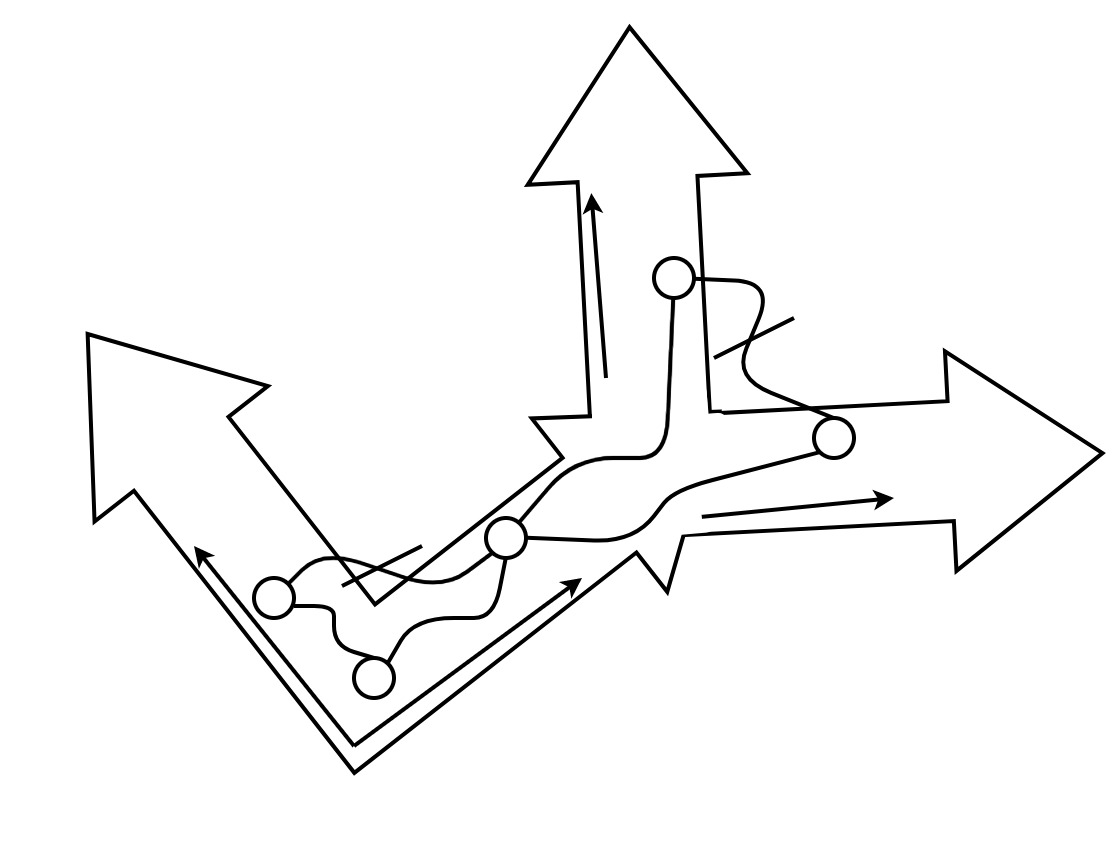
\includegraphics[width=0.5\textwidth]{sharedfutures}
\caption{Displaying the bifurcations ($n$-furcation) inheret in the statespace of estimate safety consensus protocols (with non-triviality). States with common futures (marked with $\sim$) still have the opportunity to make consistent decisions. States who don't have this opportunity don't share futures (marked with $\nsim$).}
\end{figure}

Figure 1 provides intuition about the nature of the consensus safety theorem and its contrapositive: If two nodes at two protocol states have a shared future, then they haven't made irreconcilable decisions in the $n$-furcation in protocol space. If they have made inconsistent decisions in the protocol, then they won't share a future.

The problem of consensus for us, in some way, then, is to help nodes make it to any one of any number of states with mutually exclusive safe estimates, but without losing their shared futures with other nodes in similar positions. Let us develop more language, therefore, for talking about protocol states, their safe estimates, and to their ability to evolve to states with more safe estimates.



-----------------------------------------------------------------------------------------------------------------
-----------------------------------------------------------------------------------------------------------------
-----------------------------------------------------------------------------------------------------------------
-----------------------------------------------------------------------------------------------------------------


Outline of remainder of part 1:

define bivalence 

talk about locking, give some results for locking (maybe w sketch proof)

show locked on locked on = locked on
show that anything not locked on with a morphism into locked on also has a morphism not locked on.
show that decisions on locked on are consensus safe if we share future

Bring in stuck-freeness:
  there is a path to S(p) or there is a path to S(not p) (or both).

show choose 1 of 3: locked on S(p), locked on S(not p), and bivalent (locked on S(p) union S(not p))

Wrap up:
Talk more about the safety proof, and what it means, and what we know

Then transition to Part 2:
Talk a bit about nodes and about why we need to talk about nodes (how do we really guarantee ``with something in the protocol" that nodes will make the same?)
Talk about how that would look like for a protocol to be bft using this construction


\section{Part 2: Nodes, their interaction, and Byzantine faults}

The definition of protocol executions in Part 1 does not include nodes, or their interaction. As we have just seen, it is hard to justify why nodes would make the same decision unless they are receiving messages from ``the same set" of nodes.

We will therefore go for the traditional route and assume that we have (hard-coded) consensus on ``the set of consensus-forming nodes". We are going to do this by insisting on the following:

\begin{defn}[Estimate Safety Consensus Protocols, Part 4 of ?: Nodes Running in Parallel]
\begin{description}

Protocol states $\sigma \in ob(\cat{\Sigma^1})$ satisfy one of the following:

\begin{align*}
  \sigma &= (\sigma_1,\sigma_2,\sigma_3,...,\sigma_{n-1},\sigma_n)\\
\end{align*}

And from now on, $\sigma_i$ will refer to the i'th entry of the tuple $\sigma$, \emph{which is a protocol state in another category $\cat{\Sigma}$}.

And the protocol state transitions $mo(\cat{\Sigma^1})$ satisfy:

$$
\sigma \to \sigma' \implies \sigma_i \to \sigma'_i \hspace{3mm} \forall i=1...n
$$

We will now pause the definition for further analysis again.

\end{description}
\end{defn}

The objects in the category $\cat{\Sigma^1}$ are tuples of protocol states in another category $\cat{\Sigma}$. $\cat{\Sigma}$ still enjoys the benefits of the safety proof. $\cat{\Sigma^1}$'s morphisms currently allow independent protocol executions of $\cat{\Sigma}$. It would certainly be more convenient if the morphisms in $\cat{\Sigma^1}$ guaranteed that their source and domain (the states of $\cat{\Sigma^1}$ they morph from and to) had protocol states from $\cat{\Sigma}$ with consensus safety.

\begin{defn}[Estimate Safety Consensus Protocols, Part 5 of ?: Nodes Running in Parallel with Consensus Safety]
\begin{description}

We now require that the protocol state transitions $mo(\cat{\Sigma^1})$ satisfy an additional constraint:

For $\sigma$, $\sigma'$ in $ob(\cat{\Sigma^1})$:
\begin{align*}
  \sigma \to \sigma' &\implies \sigma_i \to \sigma'_i \hspace{3mm} \forall i=1...n\\
  \sigma \to \sigma' &\implies \sigma_i \sim \sigma_j \hspace{3mm} \forall i=1...n, j=1...n\\
  \sigma \to \sigma' &\implies \sigma'_i \sim \sigma'_j \hspace{3mm} \forall i=1...n, j=1...n
\end{align*}

\end{description}
\end{defn}

Now we have restricted the consensus protocol executions only to ones that have consensus safety. However, we have not yet indicated in any way that nodes are able to communicate. We just (somewhat artificially) restricted the protocol executions of nodes (who are being modelled by entries in tuples which are objects of our category $\cat{\Sigma}$) to guarantee they won't experience consensus failure.

Unfortunately there's nothing in our model right now for communication. But at least we do know that the category $\cat{\Sigma^1}$ of consensus safe protocol executions of $\cat{\Sigma}$ also satisfies our consensus safety proof. So, lets run nodes who use that category as a protocol in parallel and see what happens:


\begin{defn}[Estimate Safety Consensus Protocols, Part 6 of ?: Adding Communication]
\begin{description}


Protocol states for a new category of protocol states $\cat{\Sigma^2}$, $\sigma \in ob(\cat{\Sigma^2})$, will satisfy the following:

\begin{align*}
  \sigma &= (\sigma_1,\sigma_2,\sigma_3,...,\sigma_{n-1},\sigma_n)
\end{align*}

This time with $\sigma_i \in \cat{\Sigma^1}$ 

And the protocol state transitions $mo(\cat{\Sigma^2})$ satisfy:

$$
\sigma \to \sigma' \land \sigma \neq \emptyset \implies \sigma_i \to \sigma'_i \hspace{3mm} \forall i=1...n
$$

We will now pause the definition for further analysis again.

\end{description}
\end{defn}

Lets review some things, quickly: 

\begin{itemize}
\item $\cat{\Sigma^2}$ is the category of $n$ parallel nodes executing protocol $\cat{\Sigma^1}$,
\item $\cat{\Sigma^1}$ is the category of $n$ parallel nodes executing protocol $\cat{\Sigma}$, without consensus failure 
\end{itemize}

So  $\cat{\Sigma^2}$ is the category of $n$ nodes watching $n$ nodes execute $\cat{\Sigma}$ while maintaining common futures

Do the morphisms in $\cat{\Sigma^2}$ evidence exactly $n$ parallel protocol executions of $\cat{\Sigma}$? Not necessarily. 

Specifically, it's possible given the definition we have so far for us to have an object $\sigma$ such that we have:

$$
\sigma_{ik} \nleftrightarrow \sigma_{jk} \iff \neg{(\sigma_{ik} \to \sigma_{jk} \lor \sigma_{jk} \to \sigma_{ik})}
$$

Or for it to have a morphism with two objects $\sigma \to \sigma'$:

Then we know that 

$$
\sigma_{ik} \to \sigma'_{ik} \land \sigma_{jk} \to \sigma'_{jk} 
$$

but 

$$
\sigma_{ik} \nleftrightarrow \sigma_{jk} \lor \sigma'_{ik} \nleftrightarrow \sigma'_{jk} \lor \sigma_{ik} \nleftrightarrow \sigma'_{jk} \lor \sigma_{jk} \nleftrightarrow \sigma'_{ik}
$$

So just as we can have an object in $\cat{\Sigma^2}$ that has objects at indeces $*k$ in $\cat{\Sigma}$ which can't have appeared from a single execution in $\cat{\Sigma}$, we can have a mophism in $\cat{\Sigma^2}$ which maps one state to another which together have objects at indeces $*k$ which can't have appeared from a single execution in $\cat{\Sigma}$.

For example, if neither of the dashed arrows in the following diagram exist, then nodes $i$ and $j$ could not have been watching the same ``node" $k$.

\begin{equation*}
\begin{tikzcd}
\sigma'_ik
  \arrow[rrrddd,dashed]
  &
{}
  &
{}
  &
\sigma'_jk
  \arrow[lllddd,dashed]
  \arrow[lll,""]
  \\ 
{}
  &
{}
  &
{}%  \arrow[r,Rightarrow,""]
  &
{}
  \\ 
{}
  &
{}
  &
{}%  \arrow[r,Rightarrow,""]
  &
{}
  \\
\sigma_ik
  \arrow[uuu,""]
  &
{}
  &
{}%  \arrow[r,Rightarrow,""]
  &
\sigma_jk
  \arrow[uuu,""]
  \arrow[lll,""]
\end{tikzcd}
\end{equation*}

\begin{defn}[Estimate Safety Consensus Protocols, Part 6 of ?: Getting rid of Equivocation]
\begin{description}


Protocol states for the category $\cat{\Sigma^2}$, $\sigma \in ob(\cat{\Sigma^2})$, will now also satisfy the following:

$$
\forall i,j,k \hspace{1mm} . \hspace{1mm} \sigma_{ik} \leftrightarrow \sigma_{jk}
$$

And the protocol state transitions $mo(\cat{\Sigma^2})$ additionally now need to satisfy:

For $\sigma \to \sigma'$:
\begin{align*}  
  \forall k \hspace{1mm} . \hspace{1mm} &\exists \{\tau_i \in mo(\cat{\Sigma})\}_{i=1}^N \text{ such that the path } \sigma_{*1} \xrightarrow[]{\tau_1} \sigma_{*2} \xrightarrow[]{\tau_3} \sigma_{*3} \xrightarrow[]{\tau_4} \sigma_{*4}... \xrightarrow[]{\tau_N} \sigma_{*N} \\
  &\text{ contains each term in $\sigma$ or $\sigma'$ of the form $\sigma_{ik}$ or $\sigma'_{ik}$, respectively, with} \\
  &\text{ $\sigma_{ik}$ not appearing after $\sigma'_{ik}$ in path $\{\tau_i \in mo(\cat{\Sigma})\}_{i=1}^N$ }
\end{align*}

I.e. there exists a (single threaded) execution of protocol states $\sigma_ij$ or $\sigma'_ij$ with last index $j = k$ which passes in the direction of $\sigma_{ik} \to \sigma'_{ik}$. 

The purpose of this condition is to restrict $\cat{\Sigma^2}$ to parallel executions of $\cat{\Sigma^1}$ which each observe ``the same" parallel execution of $\Sigma$.
\end{description}
\end{defn}

Lets do some more review: 

\begin{itemize}
\item $\cat{\Sigma^2}$ is the category of $n$ parallel nodes executing protocol $\cat{\Sigma^1}$, without equivocation
\item $\cat{\Sigma^1}$ is the category of $n$ parallel nodes executing protocol $\cat{\Sigma}$, without consensus failure 
\end{itemize}

So, a transition in $\cat{\Sigma^2}$ has the following properties:

It takes 

n nodes who are watching n nodes safely execute a consensus protocol...

...to...

n nodes each of which have new states of n nodes executing a consensus protocol.



Lets suppose that we achieve safety for a node at $\sigma_{ij} \in \cat{\Sigma}$....

Then it doesn't break consensus safety of $\sigma_i$
In fact it locks every $\sigma_ik$ to that outcome [proof required]...

And because additionally every different node in $\sigma$ is observing the same execution of $\cat{\Sigma^2}$, we know also that every $\sigma_jk$ is also locked to that outcome [proof required]

The conclusion is that $S(p,\sigma_{ij}) \implies Locked(\sigma_kl, \{\sigma': S(p,\sigma')\})$

--------

so it would be great if we could guarantee that nodes execute $\cat{\Sigma}$ without consensus failure and without equivocation. Well, we happen to know that by "without consensus failure" we mean $\sim$, which can be achieved by finding a possible future.

-------

maybe we can show that without equivocation there is always a shared future?
maybe < k faults \implies \sim?


------

in the end we want a protocol that:

detects equivocation and doesn't transition if there's too much

like if $\cat{\Sigma^2}$ allowed some equivocation, but not too much


How do the estimators relate?!?


--------------------------------------------------------------------

Outline for part 2:

Okay lets have objects be tuples of objects

Justify why this will model nodes running the protocol, while also modelling the protocol itself

Restrict morphisms so they are the same nodes

(or so they have some amount of byzantine faults (perhaps by weight))

show this can be implemented in a correct-by-construction manner with message collection and fault detection
maybe good entry point for "we always have a common future state, but it may not be byzantine free enough for us to get there"
which maybe can lead to the whole unions and deterministic functions of views thing.

Talk about initial protocol states

Talk about how we unified states of the protocol and states of nodes running the protocol



Justify that the original definition is still satisfied

Show that nodes have consensus safety
Show that $S(p, \sigma_1) \implies Locked on S(p, \sigma_2)$ if validator 1 and 2 keep a common future

Show that non-triviality and stuck-freeness can still hold

Talk about the importance of a ``good estimator" for non-triviality and stuck-freeness

Latest messages only
Follow-the-weights

Maybe we can generally use something like:
$$
\mathcal{E}(\sigma) = {argmax}_{p\in \mathcal{L}_\cat{C}} \sum_{c \in \cat{C}} \sum_{i=1}^n W(i)*(\mathcal{E}(\sigma_i)(c) \land p(c))
$$ 

But in practice we use some more tractable things.

------------------------------------------------------------------------
what about safety oracles?



----------------------------------------------------------------

Outline for part 3:

Spec casper the friendly binary consensus
Spec casper the friendly ghost

Give data


----------------------------------------------------------------






\iffalse


So our protocol states are a lot more structured, than what we knew before (only that it was a category with at least one $n$-furcation for $n\geq 2$). We may want to do some sanity checks.

------------------------------------------------------------------------------------------------------------------------------------------------------------------------------------------------------------------
------------------------------------------------------------------------------------------------------------------------------------------------------------------------------------------------------------------
------------------------------------------------------------------------------------------------------------------------------------------------------------------------------------------------------------------
------------------------------------------------------------------------------------------------------------------------------------------------------------------------------------------------------------------
------------------------------------------------------------------------------------------------------------------------------------------------------------------------------------------------------------------
------------------------------------------------------------------------------------------------------------------------------------------------------------------------------------------------------------------
------------------------------------------------------------------------------------------------------------------------------------------------------------------------------------------------------------------
------------------------------------------------------------------------------------------------------------------------------------------------------------------------------------------------------------------
------------------------------------------------------------------------------------------------------------------------------------------------------------------------------------------------------------------
------------------------------------------------------------------------------------------------------------------------------------------------------------------------------------------------------------------
------------------------------------------------------------------------------------------------------------------------------------------------------------------------------------------------------------------
------------------------------------------------------------------------------------------------------------------------------------------------------------------------------------------------------------------

\fi

TO DO:
\begin{itemize}

\item So why do we care about $\neg(S(p,\sigma_1) \land S(\neg{p},\sigma_2))$ or $S(p,\sigma_1) \implies \neg{S(\neg{p},\sigma_2)}$?

\item Tell me about non-triviality and failure modes, plox

\item Can we get some drawings?

\item How is this a consensus protocol? Or how is it related to a consensus protocol?

\item How about nodes? What is a network?

\item What about stuck-free ness and locks?

\item What about liveness m8?
\end{itemize}


\iffalse

Definition for non-stuck: sigma has a path to either [locked on] s p or [locked on] s not p

if i have both i'm bivaluent

if i have only one (say p), i'm locked on p
  because if i had a future in locked S(not p), then i would have one both
  because if i have a future which doesn't go to the one i'm on and also doesn't go to the other
  then that future is stuck


so non-stuck means not locked on S p and not locked on S not p => has path to S p and path to S not p



A stronger definition of non-triviaity:

for all sigma, p s.t. not S(p, sigma) and not S(not p, sigma) => sigma has path to sigma' S(p, sigma') and path to sima'' st S(not p, sigma')

This one is:
  non-stuckness
  bi-valence
  non-triviality (if exists states wth unsafe p and unsafe not p)
  taming complexity (no states locked on s p which are not in s p)

Do we want to show there exist safe states outside of non-triviality?
Do we need more aggressive non-triviality?
where for every object either safe on p or safe on not p or has path to S(p) and a path to S(not (p))?
Ideally also non-stuckness?


------------------------------------------------ RAMBLE RAMBLE RAMBLE --------------------------------------------------------------


non-stuckness and bivalence

if a node is safe on p
another is not safe on not p (by shared futures)

but that other also:
1) has a path to safe on p (by shared futures)
2) has no path to safe on not p (IF THEY MAINTAIN SHARED FUTURES (A HIGHER ORDER PROPERTY NOT DEFINED YET!))
3) is not locked off safe on p (bc they share future)
4) has no path to locked off safe p (bc they share future)
???
6) locked on S(p)





So, WTS 

sigma ~ sigma' OVER TIME
no stuckness

==>

S(p, sigma) => locked on S(p), simga'

When does locked on safety -> safety? 

When being on not p means that you have a path to S (not p).

Do we get this from extended non-triviality?

not safe on not p and not safe on p => have a path to both S(p) and S(not p)?

So locked on(S(p),s) -> S(p, s)

or would we want non-triviality to talk about locks on safety rather than safety?

What would be the benefit?

I could re-write E to change all mappings E(sigma) => p to E(sigma) => not p, when locked on S(not p, sigma).

So what's the easiest way to get rid of set difference locked on S \ S?

E(sigma) => p implies exists sigma -> sigma' s.t. S(p, sigma')

or

not S(p) and not S(not p) => path to S(p) and path to S(not p)

This one is quite strong 

its' 

non-stuckness and bi-valence
non-triviality (if exists states wth unsafe p and unsafe not p)
taming complexity (no states locked on s p which are not in s p)

------------------------------------------------ RAMBLE RAMBLE RAMBLE --------------------------

i can show the bivalance of states which are not locked on s p and not locked on s not p if i have non-stuckness


non-stuck : i have a path to either locked on s p or locked on s not p

if i have both i'm bivaluent

if i have only one (say p), i'm locked on p
  because if i had a future in locked S(not p), then i would have one both
  because if i have a future which doesn't go to the one i'm on and also doesn't go to the other
  then that future is stuck


so non-stuck means not locked on S p and not locked on S not p => has path to S p and path to S not p





ALTERNATIVELY



We can refactor to use locked on S(p) for decisions and non-triviality

not L(S(p)) and not L(S(not p)) => path to L(S(p)) and path to L(S(not p))




Are we going to need a fork choice rule separate from estimator?

E(F(s))

in order to show that there are safe states that they can reach in the context of mad forking in the monoidal version?

Well, we have safety either way..



\fi



\iffalse




------------------------------------------------------------------------------------------------------------------------------------------------------------------------------------------------------------------
------------------------------------------------------------------------------------------------------------------------------------------------------------------------------------------------------------------
------------------------------------------------------------------------------------------------------------------------------------------------------------------------------------------------------------------
------------------------------------------------------------------------------------------------------------------------------------------------------------------------------------------------------------------
------------------------------------------------------------------------------------------------------------------------------------------------------------------------------------------------------------------
------------------------------------------------------------------------------------------------------------------------------------------------------------------------------------------------------------------
------------------------------------------------------------------------------------------------------------------------------------------------------------------------------------------------------------------
------------------------------------------------------------------------------------------------------------------------------------------------------------------------------------------------------------------
------------------------------------------------------------------------------------------------------------------------------------------------------------------------------------------------------------------
------------------------------------------------------------------------------------------------------------------------------------------------------------------------------------------------------------------
------------------------------------------------------------------------------------------------------------------------------------------------------------------------------------------------------------------
------------------------------------------------------------------------------------------------------------------------------------------------------------------------------------------------------------------
------------------------------------------------------------------------------------------------------------------------------------------------------------------------------------------------------------------
------------------------------------------------------------------------------------------------------------------------------------------------------------------------------------------------------------------
------------------------------------------------------------------------------------------------------------------------------------------------------------------------------------------------------------------
------------------------------------------------------------------------------------------------------------------------------------------------------------------------------------------------------------------
------------------------------------------------------------------------------------------------------------------------------------------------------------------------------------------------------------------
------------------------------------------------------------------------------------------------------------------------------------------------------------------------------------------------------------------
------------------------------------------------------------------------------------------------------------------------------------------------------------------------------------------------------------------
------------------------------------------------------------------------------------------------------------------------------------------------------------------------------------------------------------------
------------------------------------------------------------------------------------------------------------------------------------------------------------------------------------------------------------------
------------------------------------------------------------------------------------------------------------------------------------------------------------------------------------------------------------------
------------------------------------------------------------------------------------------------------------------------------------------------------------------------------------------------------------------
------------------------------------------------------------------------------------------------------------------------------------------------------------------------------------------------------------------
------------------------------------------------------------------------------------------------------------------------------------------------------------------------------------------------------------------
------------------------------------------------------------------------------------------------------------------------------------------------------------------------------------------------------------------
------------------------------------------------------------------------------------------------------------------------------------------------------------------------------------------------------------------
------------------------------------------------------------------------------------------------------------------------------------------------------------------------------------------------------------------
------------------------------------------------------------------------------------------------------------------------------------------------------------------------------------------------------------------
------------------------------------------------------------------------------------------------------------------------------------------------------------------------------------------------------------------

\fi

\iffalse



Nodes following estimate safety consensus protocols only make decisions on propositions $p$ when they are in a state $\sigma$ such that $S(p,\sigma)$.

If two nodes with states $\sigma_1$ and $\sigma_2$ with $\sigma_1 \sim \sigma_2$ each make decisions on any number of safe propositions $P_{\sigma_1} = \{p: S(p,\sigma_1)\}$ and $P_{\sigma_2} = \{p: S(p,\sigma_2)\}$, then the nodes have consistent safe propositions, at least in the sense that:

\begin{align*}
\nexists p_1 \in P_{\sigma_1} \hspace{1mm} &. \hspace{1mm} \land_{q \in P_{\sigma_2}} q \implies \neg{p_1} \\
\nexists p_2 \in P_{\sigma_2} \hspace{1mm} &. \hspace{1mm} \land_{q \in P_{\sigma_1}} q \implies \neg{p_2}
\end{align*}



\pagebreak
\pagebreak



Before level 2 we might consider:

\section{Safety Proof: Level 2}



\begin{equation}
\begin{tikzcd}
A \arrow[r,"f"]
  \arrow[dr,swap,"g\circ f"]
  &
B \arrow[dr,"g\circ h"]
  \arrow[d,swap,"g"]
  \\
  {}&
C \arrow[r,swap,"h"]
  &
D
\end{tikzcd}
\end{equation}


\begin{equation*}
\begin{tikzcd}
{}
  &
\sigma_3
  &
{}
  \\ 
\sigma_1
  \arrow[ur,""]
  &
{}
  &
\sigma_2
  \arrow[ul,""]
\end{tikzcd}
\end{equation*}



\fi









































































\iffalse



\section{Introduction}
Traditional consensus protocols (such as multi-Paxos and pbft) are notoriously difficult to understand. This difficulty arises largely from the fact that these protocols were derived to satisfy a non-local safety property.

The Bitcoin blockchain, on the other hand, is famously easy to understand. This ease comes partly from the simplicity of the specification, but it also arises from the local nature of ``confirmations".

This work will be organized as follows: First, we will provide elementary definitions and proofs which will relate consensus protocols of the new "blockchain variety" to protocols of the "traditional variety". Secondly, we will give two consensus protocols that meaningfully satisfy these definitions and proofs. Finally, we will show that these protocols have efficient, practical implementions.

The writing style will be informal because our aim is to help novice readers learn about consensus protocols, not to be a part of the academic literature.

\section{Foundational Definitions and Theorem}

Consensus protocols are fundamentally about having \emph{nodes} who run the protocol make the same decisions. Nodes that follow the protocol are called ``correct" or ``protocol-following". 

Consensus is challenging because each node is a different location in a distributed system, and therefore may see different protocol messages in different orders. It is sometimes additionally complicated because we often want to acheive consenssu in the presence of nodes who might crash (``crash-faulty nodes'') or nodes who might not be following the protocol at all (``Byzantine nodes'').

A ``decision" can be understood as an irreversible commitment. Once a node decides on ``a value of the consensus'', it cannot later decide on a different value. Decisions have classically been considered to be the output of a consensus protocol.

\begin{defn}[Consensus safety]
A consensus protocol is said to be ``safe” if any two correct nodes, having each made a decision, decided on the same value.
\end{defn}

All traditional consensus protocols have been derived to satisfy this definition.

The Bitcoin blockchain protocol, on the other hand, does not explicitly make decisions. However, it does still \emph{act} like a consensus protocol because it lets people interacting with the blockchain make the same decision. All they have to do is wait for 6 confirmations!

An ``estimate'' can be understand as a reversible guess. A node who makes an estimate on a value of the consensus may at a later stage of the protocol have an estimate with a different value. 

\begin{defn}[Estimate safety]
A correct node's estimate is said to be ``safe'' if that node will not have a different estimate in any future protocol state.
\end{defn}

The following theorem is fundamental:

\begin{thm}[Estimate safety $\implies$ Consensus safety]
If two correct nodes who receive the same set of protocol messages have the same estimates regardless of message arrival order, and any correct nodes can receive any protocol messages, then decisions on safe estimates have consensus safety.
\end{thm}

It relates consensus protocols that make estimates to those that make decisions through the operation of deciding on safe estimates (at least for protocols where estimates are independent of message arrival order, and where any node can potentially receive any protocol message).

\begin{proof}
Lets assume that correct node $A$ has safe estimate $e_A$ and has received protocol messages $m_A$, and that node correct $B$ has safe esitmate $e_B$ and has received protocol messages $m_B$.

If $B$ were to receive messages $m_A$, and $A$ were to receive messages $m_B$, then $A$ and $B$ would both have received protocol messages $m_A \cup m_B$. At this point, $A$ and $B$ would have the same estimate, by virtue of having each received the same protocol messages.

However, neither $A$ nor $B$ would have changed their estimates after receiving messages $m_B$ or $m_A$, respectively, because their estimates are safe.

This must mean that $e_A = e_B$, completing the proof.

\end{proof}

This proof, however, does not say anything about whether there exist protocols for detecting estimate safety. The following section will give examples of a couple of estimate safety consensus protocols.

\section{Protocol Specifications}

The protocols that we're going to see here have a few things in common. First, there is a fixed set of nodes $V$ (called ``validators'') who are responsible for originating protocol messages. 

Each of these valdiators have ``weights", implemented by a map (which is part of the protocol specification, at least for now):

$$
W: V \to \mathbb{R}_+
$$

which has the ``tie breaking property":

$$
\sum_{v \in V_1} W(v) \neq \sum_{v \in V_2} W(v), \forall V_1 \neq V_2 \subseteq V
$$

Additionally, messages have the following form:

$$
M = E \times V \times J
$$

Where $E$ is the ``estimate space'', which contains all possible estimate values, or the possible values of the consensus. $V$ is the set of validators, as before. $J$ is the set of ``justifications", which we will understand for now as a (possibly empty) set of protocol messages

A message $m_1$ is a ``dependency" of a message $m_2$ if it is in the justification of $m_2$, or if it a dependency of any messages in the justification of $m_2$. Put another way, $m_1$ is a dependency of $m_2$ if it's in the closure under set membership in the justification of $m_2$

Two messages $m_1$ and $m_2$ are called ``an equivocation" if they are from the same validator but neither are a dependency of the other. In each of these protocols, producing an equivocation is considered Byzantine behaviour.

``Protocol states", also called ``views", for each of these protocols, consist simply of sets of protocol messages. 

A message $m_1$ from validator $v$ is a ``latest message" in a view $u$ if there is no $m_2 \in u$ from validator $v$ such that $m_1$ is a depednency of $m_2$.

Finally, each of these protocols have deterministic ``estimators", which are functions that map protocol states to estimates:

$$
\mathcal{E}: \mathcal{P}(M) \to E\cup\emptyset
$$

The estimators are a function only of the latest messages in the estimator's view with senders who are not equivocating in that view. It returns $\emptyset$ if and only if there are no such latest messages.

A protocol message is called ``valid" if the estimator of its justiication returns $\emptyset$ or the message's estimate. We'll assume that all protocol messages are valid.

\subsection{Casper the Friendly Binary Consensus}

For the binary consensus, the estimator is max weight given latest messages.

\subsection{Casper the Friendly Ghost}

For the blockchain consensus, the estimator is GHOST given latest messages


\subsection{Efficient safety determination}

1.
2.
3.

\subsection{Liveness}

\subsection{Validator rotation for the }

\section{Simulation}


\fi



\iffalse

\begin{proof}
  \begin{align*}
    \sigma \to \sigma' \land S(p,\sigma)& \implies\\
    \sigma \to \sigma' \land S(p,\sigma)& \land \sigma' \to \sigma'' \\
    \iff \sigma \to \sigma' \land S(p,\sigma)& \land \sigma' \to \sigma'' \land \sigma \to \sigma'' &&\text{(morphism composition)} \\
    \implies \sigma \to \sigma' \land S(p,\sigma)& \land \sigma' \to \sigma'' \land \sigma \to \sigma'' \land \mathcal{E}(\sigma'') \Rightarrow p  &&\text{(using Lemma)} \\
    \iff \sigma \to \sigma' \land S(p,\sigma)& \land \sigma' \to \sigma'' \land \mathcal{E}(\sigma'') \Rightarrow p \\
    \implies \sigma \to \sigma' \land S(p,\sigma)& \land \sigma' \to \sigma'' \implies \mathcal{E}(\sigma'') \Rightarrow p  \\
    \implies \sigma \to \sigma' \land S(p,\sigma)& \implies( \sigma' \to \sigma'' \implies \mathcal{E}(\sigma'') \Rightarrow p ) \\
    \iff \sigma \to \sigma' \land S(p,\sigma)& \implies S(p, \sigma') \\
    \sigma \to \sigma' \land S(p,\sigma) \implies \sigma \to \sigma' \land S(p,\sigma) \implies S(p, \sigma') \\
    \iff \sigma \to \sigma' \land S(p,\sigma) \implies S(p, \sigma') &&\qedhere
  \end{align*}
\end{proof}

\begin{proof}
  \begin{align*}
    S(p,\sigma) &\iff \sigma \to \sigma' \implies \mathcal{E}(\sigma') \Rightarrow p &&\text{(applying the definition)} \\
    &\implies \sigma' \to \sigma'' \land \sigma \to \sigma' \implies \mathcal{E}(\sigma') \Rightarrow p
    \sigma' \to \sigma'' \land \sigma \to \sigma' &\implies \sigma \to \sigma''
    \sigma \to \sigma'' \implies \mathcal{E}(\sigma'')


    \sigma \to \sigma' \land S(p,\sigma)
    \sigma \to \sigma' \land \sigma \to \sigma'' \implies \mathcal{E}(\sigma'') 


    \sigma \to X \land S(p,\sigma)
    \sigma \to X \land 


    Lemma:


    Ideal proof flow:




    \sigma \to \sigma' \land \sigma' \to X \implies \sigma \to X


    \sigma \to \sigma' \land S(p,\sigma) \implies \sigma' \to X \implies \mathcal{E}(X) \Rightarrow p
    \sigma \to \sigma' \land S(p,\sigma) \implies S(p,\sigma')


    \forall{\sigma''}. \hspace{1mm} \sigma' \to \sigma'' \land \mathcal{E}(\sigma') \Rightarrow p \hspace{5mm}  \land \forall{\sigma'}. \hspace{1mm} \sigma \to \sigma \\
    &\implies \mathcal{E}(\sigma') \Rightarrow p \hspace{5mm} \forall{\sigma', \sigma''}. \hspace{1mm} \sigma \to \sigma' \land \sigma' \to \sigma''  \\
    &\implies \mathcal{E}(\sigma'') \Rightarrow p \hspace{5mm} \forall{\sigma', \sigma''}. \hspace{1mm} \sigma \to \sigma' \land \sigma' \to \sigma'' &&\text{(using $\sigma \to \sigma''$, from composition)} \\
    &\implies \mathcal{E}(\sigma'') \Rightarrow p \hspace{5mm} \forall{\sigma''}. \hspace{1mm} \sigma' \to \sigma'' \land \forall{\sigma'}. \hspace{1mm} \sigma \to \sigma'  \\
    &\implies S(p, \sigma') \hspace{5mm} \forall{\sigma'} \hspace{1mm} . \hspace{1mm} \sigma \to \sigma'\\
    &\implies \sigma \to \sigma' \implies S(p, \sigma') \\
    S(p,\sigma) &\land \sigma \to \sigma' \implies S(p, \sigma') &&\qedhere
  \end{align*}
\end{proof}


\begin{proof}
  \begin{align*}
    S(p,\sigma) &\iff \mathcal{E}(\sigma') \Rightarrow p \hspace{5mm} \forall{\sigma'}. \hspace{1mm} \sigma \to \sigma' &&\text{(applying the definition)} \\
    \sigma' \to \sigma'' \land \mathcal{E}(\sigma') \Rightarrow p \hspace{5mm}  \land \forall{\sigma'}. \hspace{1mm} \sigma \to \sigma' \\
    &\implies \mathcal{E}(\sigma') \Rightarrow p \hspace{5mm} \forall{\sigma', \sigma''}. \hspace{1mm} \sigma \to \sigma' \land \sigma' \to \sigma''  \\
    &\implies \mathcal{E}(\sigma'') \Rightarrow p \hspace{5mm} \forall{\sigma', \sigma''}. \hspace{1mm} \sigma \to \sigma' \land \sigma' \to \sigma'' &&\text{(using $\sigma \to \sigma''$, from composition)} \\
    &\implies \mathcal{E}(\sigma'') \Rightarrow p \hspace{5mm} \forall{\sigma''}. \hspace{1mm} \sigma' \to \sigma'' \land \forall{\sigma'}. \hspace{1mm} \sigma \to \sigma'  \\
    &\implies S(p, \sigma') \hspace{5mm} \forall{\sigma'} \hspace{1mm} . \hspace{1mm} \sigma \to \sigma'\\
    &\implies \sigma \to \sigma' \implies S(p, \sigma') \\
    S(p,\sigma) &\land \sigma \to \sigma' \implies S(p, \sigma') &&\qedhere
  \end{align*}
\end{proof}




\begin{proof}
  Assuming that $S(p,\sigma)$, we aim to show that $\neg{S(\neg{p},\sigma)}$
  \begin{align*}
    &\sigma \to \sigma' \implies \mathcal{E}(\sigma') \Rightarrow p &&\text{(by assumption $S(p, \sigma)$ and definition of $S$) }   &&\text{(1)} \\
    &\sigma \to \sigma &&\text{(by the existence of the identity morphism  $\sigma \xrightarrow[]{\tau_0} \sigma$} &&\text{(2)} \\
    &\mathcal{E}(\sigma) \Rightarrow p &&\text{(by (1) and (2))} &&\text{(3)}\\
    &S(\neg{p},\sigma) \implies \mathcal{E}(\sigma) \Rightarrow \neg{p} &&\text{(using the identity morphism and the definition of $S$, not unlike in (3))}   &&\text{(4)} \\
    \neg{(\mathcal{E}(\sigma) \Rightarrow \neg{p})} \implies \neg{S(\neg{p},\sigma)} &&\text{(the contrapositive of (4))}  &&\text{(5)} \\
    \mathcal{E}(\sigma) \Rightarrow p \implies \neg{(\mathcal{E}(\sigma) \Rightarrow \neg{p})} &&\text{(this is a property of $\mathcal{E}$ for any argument, by definition)}  &&\text{(6)} \\
    \neg{S(\neg{p},\sigma)} &&\text{(from (3), (6) and (5)) }   &&\text{(7)} &&\qedhere
 

    \neg{\neg{\mathcal{E}} \lor \neg{p}}
    mathcal{E} \land p
    mathcal{E} \Rightarrow p
    &S(p,\sigma) \implies     &\sigma \to \sigma' \implies \mathcal{E}(\sigma') \Rightarrow p &&\text{(by assumption $S(p, \sigma)$ and definition of $S$) }   &&\text{(1)} \\
    &\sigma \to \sigma' \implies \mathcal{E}(\sigma') \Rightarrow p &&\text{(by assumption $S(p, \sigma)$ and definition of $S$) }   &&\text{(1)} \\
\neg{S(\neg{p},\sigma')} &&\text{(contrapositive of (4))} &&\text{(5)} \hspace{5mm} &&\qedhere
  \end{align*}
\end{proof}



\begin{equation*}
\begin{tikzcd}
{}
  &
\sigma_3
  &
{}
  \\ 
\sigma_1
  \arrow[ur,""]
  &
{}
  &
\sigma_2
  \arrow[ul,""]
\end{tikzcd}
\end{equation*}



\fi

\end{document}
